\begin{figure}
    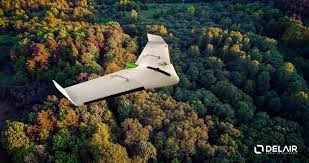
\includegraphics[width=\textwidth]{Imagenes/dron.jpg}
     \hfill
     %\caption{Superposition of manual and automatic shadow masks (red contour and blue colored area), using 60th percentile, using ψ\textsubscript{BR} (blue an red channels) for the Invariant color index}
    \label{dron}
\end{figure}

\begin{figure}
    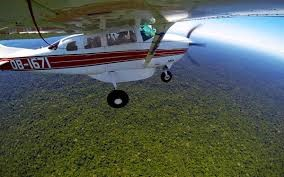
\includegraphics[width=\textwidth]{Imagenes/avion.jpg}
     \hfill
     %\caption{Superposition of manual and automatic shadow masks (red contour and blue colored area), using 60th percentile, using ψ\textsubscript{BR} (blue an red channels) for the Invariant color index}
    \label{avion}
\end{figure}

\begin{figure}
    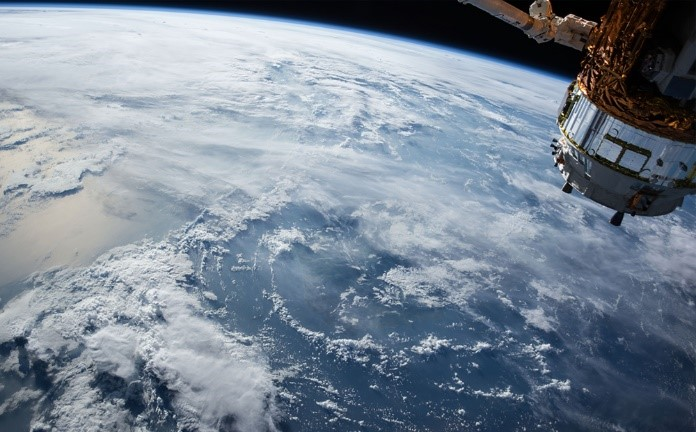
\includegraphics[width=\textwidth]{Imagenes/satelite.jpg}
     \hfill
     %\caption{Superposition of manual and automatic shadow masks (red contour and blue colored area), using 60th percentile, using ψ\textsubscript{BR} (blue an red channels) for the Invariant color index}
    \label{satelite}
\end{figure}